%%%%%%%%%%%%%%%%%%%%%%%%%%%%%%%%%%%%%%%%%%%
%%%%%%%%%%%%%%%%%%%%%%%%%%%%%%%%%%%%%%%%%%%
%%%%%%%%%%%%%%% CHAPTER 05 %%%%%%%%%%%%%%%%


\section{Modelagem: sistemas mecânicos de translação}

\frame{
\frametitle{Variáveis}
\begin{block}{Símbolos utilizados}
\begin{itemize}
    \item Os símbolos para as variáveis básicas utilizadas para descrever o comportamento de um sistema mecânico translacional são:
    \begin{itemize}
        \item $x$, \textbf{deslocamento} em metros (m)
        \item $v$, \textbf{velocidade} em metros (m/s)
        \item $a$, \textbf{aceleração} em metros por segundo ao quadrado (m/s$^2$)
        \item $f$, \textbf{força} em newtons (N)
    \end{itemize}
\end{itemize}
\end{block}
}

\frame{
\frametitle{Variáveis}
\begin{block}{Deslocamento}
\begin{itemize}
    \item Deslocamentos são medidos em relação a uma \textbf{referência}, que geralmente é a \textbf{posição de equilíbrio} do corpo ou do ponto.
    \begin{itemize}
        \item Na primeira figura, a variável $x$ representa o deslocamento do lado esquerdo do corpo a partir da parede vertical fixa.
        \item Na segunda imagem, a posição de referência correspondente a $x=0$ não é explicitamente mostrada.
    \end{itemize}
\end{itemize}
\end{block}
\vspace{0.2cm}
\centerline{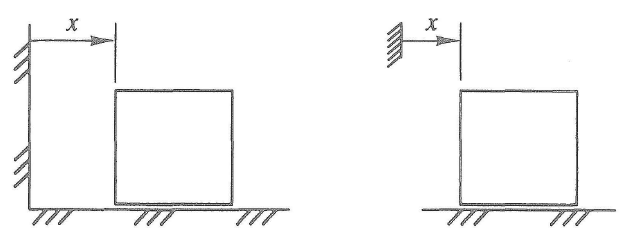
\includegraphics[width=0.7\linewidth]{Figuras/Ch05/fig1.PNG}}
}

\frame{
\frametitle{Variáveis}
\begin{block}{Velocidade}
\begin{itemize}
    \item Há duas maneiras de definir a velocidade em um sistema:
    \begin{itemize}
        \item Na primeira figura, todos os pontos do corpo em análise devem se mover a uma \textbf{mesma velocidade} $v$, portanto, não há possibilidade de ambiguidade.
        \item Na segunda imagem, a linha vertical na seta que representa o vetor velocidade indica que $v$ é a \textbf{velocidade do ponto} $A$.
    \end{itemize}
\end{itemize}
\end{block}
\vspace{0.2cm}
\centerline{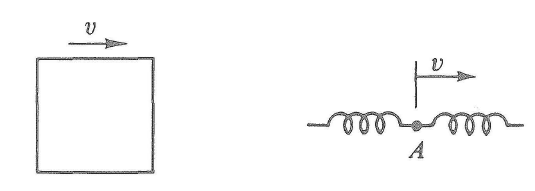
\includegraphics[width=0.7\linewidth]{Figuras/Ch05/fig2.PNG}}
}

\frame{
\frametitle{Variáveis}
\begin{block}{Força}
\begin{itemize}
    \item Uma força aplicada a um sistema pode ser representada por uma seta "entrando"\ no diagrama ou "saindo"\ dele. Ambas representações são \textbf{equivalentes}.
\end{itemize}
\end{block}
\vspace{0.2cm}
\centerline{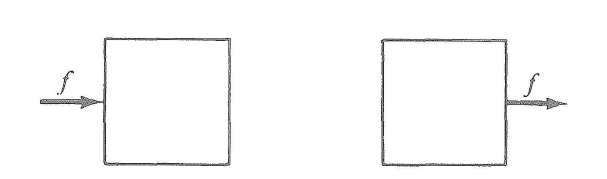
\includegraphics[width=0.7\linewidth]{Figuras/Ch05/fig3.PNG}}
}

\frame{
\frametitle{Referência x direção}
\begin{block}{Atenção}
\begin{itemize}
    \item As setas apenas indicam a posição assumida como referência para o deslocamento (ou velocidade ou força) \textbf{positivo}. Isto não implica na direção atual do movimento em um determinado instante.
    \begin{itemize}
        \item \textbf{Exemplo}: $f(t) = sen(t)$ temos que a força age para a direita (tomando como exemplo a figura do slide anterior) para $0 < t < \pi$ e depois para esquerda para $\pi < t < 2\pi$, mudando de direção a cada $\pi$ segundos.
        \item Desenhar a seta para esquerda e escrever $f(t) = -sen(t)$ é equivalente.
        \item Múltiplas soluções $\longrightarrow$ \textbf{consistência}.
    \end{itemize}
\end{itemize}
\end{block}
}

\frame{
\frametitle{Leis dos elementos}
\begin{block}{Massa}
\begin{itemize}
    \item Uma massa $\bm{M}$ (unidade de quilogramas - Kg) sujeita a uma força $f$ pode ter a sua relação escrita por meio da \textbf{segunda lei de Newton}, que diz: \textbf{"a soma das forças agindo em um corpo é igual a variação no tempo da mudança do momento"}
    $$f = \dfrac{d}{dt}(Mv)$$
Para uma massa constante, temos:
$$f = M \dfrac{dv}{dt} = M \dot{v} = Ma = M \ddot{x}$$
\end{itemize}
\end{block}
\vspace{0.1cm}
\centerline{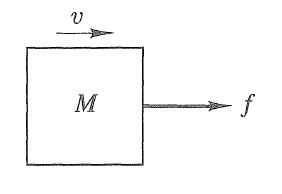
\includegraphics[width=0.3\linewidth]{Figuras/Ch05/fig4.PNG}}
}

\frame{
\frametitle{Leis dos elementos}
\begin{block}{Atrito}
\begin{itemize}
    \item Forças que são funções algébricas de \textbf{velocidades} relativas entre dois corpos são modeladas por meio de elementos \textbf{amortecedores}.
    \item Em alguns casos pode-se negligenciar tal força (última imagem). 
    \item A direção da força de \textbf{atrito} é tal que se \textbf{opõe} ao movimento da massa.
    $$f = B\Delta v$$
onde $B$ é o coeficiente de atrito (N$\cdot$s/m) e $\Delta v = v_2 - v_1$
$$f = B (v_2 - v_1)= B (\dot{x}_2-\dot{x}_1)$$
\end{itemize}
\end{block}
\vspace{0.1cm}
\centerline{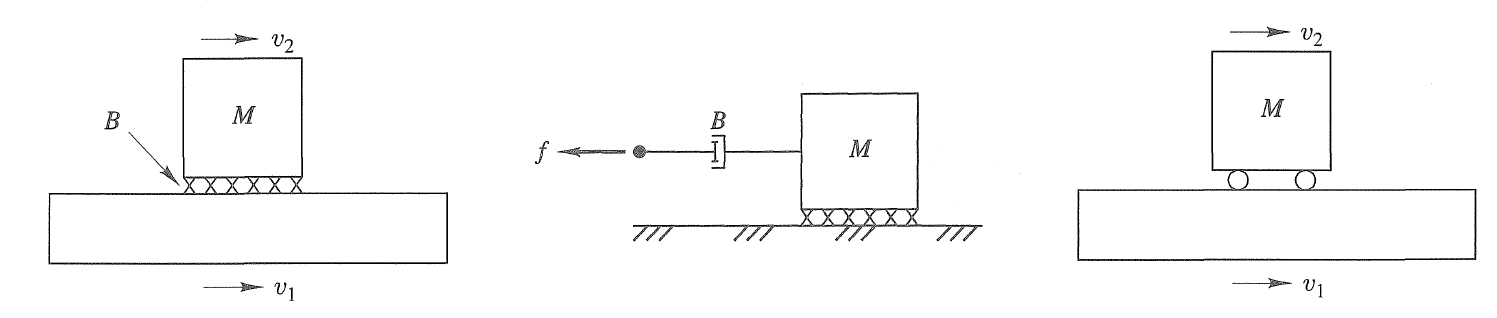
\includegraphics[width=1.05\linewidth]{Figuras/Ch05/fig5.PNG}}
}

\frame{
\frametitle{Leis dos elementos}
\begin{block}{Rigidez}
\begin{itemize}
    \item Todo elemento mecânico que está sujeito a uma mudança em sua \textbf{estrutura}, em seu formato, quando submetido à uma força pode ser comumente modelado por meio de uma \textbf{mola}.
    \item A \textbf{lei de Hooke} é a expressão matemática utilizada para calcular a força elástica exercida por um corpo que, quando deformado, tende a voltar ao seu formato original \textbf{(força restauradora)}.
$$f = K\Delta x$$
onde $K$ é a constante elástica da mola (N/m) e $\Delta x = x_2 - x_1$
$$f = K (x_2 - x_1)$$
\end{itemize}
\end{block}
}

\frame{
\frametitle{Leis dos elementos}
\begin{block}{Rigidez}
\begin{itemize}
    \item Tração
    \item Compressão
\end{itemize}
\end{block}
\vspace{0.2cm}
\centerline{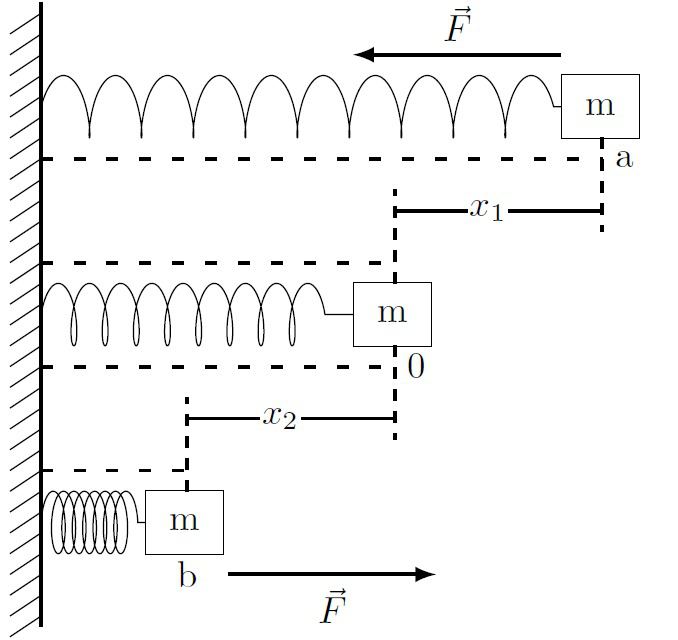
\includegraphics[width=0.5\linewidth]{Figuras/Ch05/fig6.png}}
}

\frame{
\frametitle{Interconectando as leis}
\begin{block}{Lei de D'Alembert}
\begin{itemize}
    \item A lei de D'Alembert é apenas uma reorganização da segunda lei de Newton. Ela diz que a soma dos momentos em um ponto particular P terá uma resultante nula.
    \item Considerando o nosso caso em estudo, tal lei nos diz que a soma algébrica de todas as forças aplicadas externamente em um corpo e da força de inércia (que resiste ao movimento do corpo) em uma direção particular é zero.
\end{itemize}
$$\sum_{i}^{} (f_{ext})_i = M \dfrac{dv}{dt} \implies \sum_{i}^{} (f_{ext})_i - M \dfrac{dv}{dt} = 0$$
$$\boxed{\sum_{i}^{} f_i = 0}$$
\end{block}
}

\frame{
\frametitle{Interconectando as leis}
\begin{block}{Lei de D'Alembert}
\begin{itemize}
    \item $M \dfrac{dv}{dt}$ é a \textbf{força de inércia}.
\end{itemize}
\end{block}
\vspace{0.2cm}
\centerline{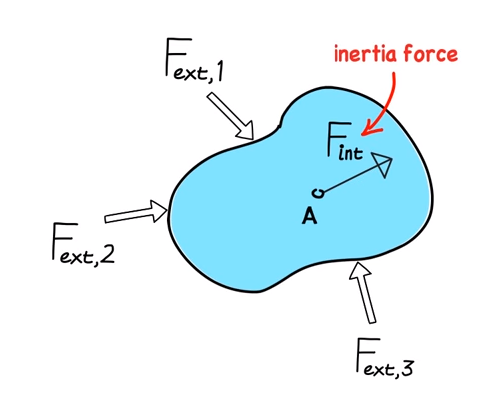
\includegraphics[width=0.5\linewidth]{Figuras/Ch05/fig7.PNG}}
}

\frame{
\frametitle{Exemplo $\#01$ - sistema massa-mola-amortecedor}
\centerline{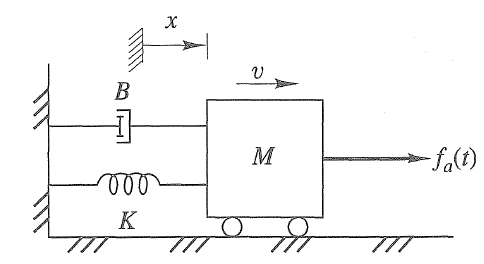
\includegraphics[width=0.4\linewidth]{Figuras/Ch05/fig8.PNG}}
\begin{block}{Problema}
\begin{itemize}
    \item Análise feita na \textbf{massa} $\bm{M}$.
    \item Movimento apenas no eixo $x$, e este da esquerda para direita.
    \item As forças horizontais são:
    \begin{itemize}
        \item $\bm{f_K}$: força exercida pela mola. Tal força restauradora deve ser para a \textbf{esquerda}, já que com o movimento de $x$ para direita, a mola é alongada. Logo, $f_k$ puxa a massa M para esquerda (ação e reação).
        \item $\bm{f_B}$: força exercida pelo amortecedor. Também para a \textbf{esquerda} visto que a velocidade está para direita.
        \item $\bm{f_I}$: força de inércia. Esta força também se encontra para a \textbf{esquerda}, se opondo ao movimento do corpo para direita.
        \item $\bm{f_a(t)}$: força aplicada ao sistema, para \textbf{direita}.
    \end{itemize}
\end{itemize}
\end{block}
}

\frame{
\frametitle{Exemplo $\#01$ - sistema massa-mola-amortecedor}
\centerline{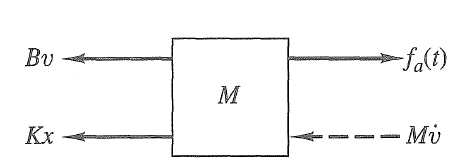
\includegraphics[width=0.5\linewidth]{Figuras/Ch05/fig9.PNG}}
\begin{block}{Diagrama de corpo livre}
\begin{itemize}
    \item Aplicando a lei de D'Alembert, \textbf{respeitando as direções assumidas}, e considerando que as forças agindo para direita são positivas, obtemos:
$$f_a(t) - (M\dot{v} + Bv + Kx) = 0$$
Substituindo $v$ por $\dot{x}$ e $\dot{v}$ por $\ddot{x}$, e rearranjando os termos, temos:
$$M\ddot{x} + B\dot{x} + Kx = f_a(t)$$
\end{itemize}
\end{block}
}

\frame{
\frametitle{Exemplo $\#02$ - sistema com duas massas interconectadas}
\centerline{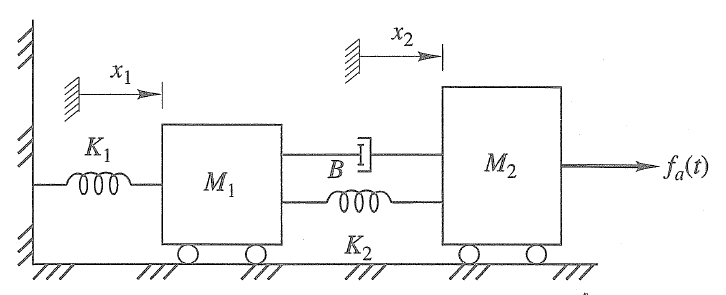
\includegraphics[width=0.6\linewidth]{Figuras/Ch05/fig10.PNG}}
\begin{block}{Problema}
\begin{itemize}
    \item A análise deve ser feita \textbf{separadamente} nas duas \textbf{massas} $\bm{M_1}$ e $\bm{M_2}$ (podem se mover com velocidades desconhecidas diferentes).
    \item Para a massa $\bm{M_1}$ \textbf{(considere} $\bm{x_2 > x_1)}$:
    \begin{itemize}
        \item A força restauradora $\bm{K_1x_1}$ atua apenas na massa 1, para a esquerda.
        \item Do mesmo modo acontece com a força de inércia $\bm{M_1\ddot{x}_1}$.
        \item A parcela $\bm{K_2(x_2-x_1)}$, considerando a mola entre as duas massas e lembrando que $x_2 > x_1$ (por hipótese), resulta em uma força de reação para direita.
        \item De modo semelhante temos $\bm{B(\dot{x}_2 - \dot{x}_1)}$ para a direita.
    \end{itemize}
\end{itemize}
\end{block}
}

\frame{
\frametitle{Exemplo $\#02$ - sistema com duas massas interconectadas}
\centerline{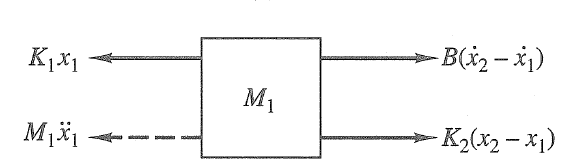
\includegraphics[width=0.5\linewidth]{Figuras/Ch05/fig11.PNG}}
\begin{block}{Diagrama de corpo livre}
\begin{itemize}
    \item Aplicando a lei de D'Alembert, \textbf{respeitando as direções assumidas}, e considerando que as forças agindo para direita são positivas, obtemos:
$$B(\dot{x}_2 - \dot{x}_1) + K_2(x_2-x_1) - M_1\ddot{x}_1 - K_1x_1 = 0$$
Rearranjando os termos, temos:
$$M_1\ddot{x}_1 + B\dot{x}_1 + (K_1 + K_2)x_1 - B\dot{x}_2 - K_2x_2= 0$$
\end{itemize}
\end{block}
}

\frame{
\frametitle{Exemplo $\#02$ - sistema com duas massas interconectadas}
\centerline{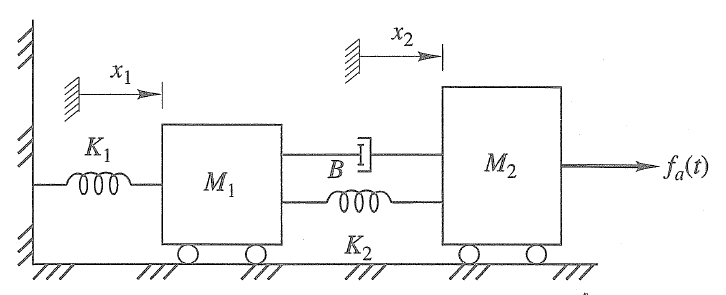
\includegraphics[width=0.6\linewidth]{Figuras/Ch05/fig10.PNG}}
\begin{block}{Diagrama de corpo livre}
\begin{itemize}
    \item A análise deve ser feita \textbf{separadamente} nas duas \textbf{massas} $\bm{M_1}$ e $\bm{M_2}$ (podem se mover com velocidades desconhecidas diferentes).
    \item Para a massa $\bm{M_2}$ \textbf{(obrigatoriamente deve-se continuar considerando} $\bm{x_2 > x_1)}$:
    \begin{itemize}
        \item A força de inércia $\bm{M_2\ddot{x}_2}$ atua para esquerda, contrária ao movimento.
        \item A parcela $\bm{K_2(x_2-x_1)}$, considerando a mola entre as duas massas e lembrando que $x_2 > x_1$ (por hipótese), resulta em uma força de reação para esquerda.
        \item De modo semelhante temos $\bm{B(\dot{x}_2 - \dot{x}_1)}$ para a esquerda.
        \item A força aplicada $f_a(t)$ está para direita.
    \end{itemize}
\end{itemize}
\end{block}
}

\frame{
\frametitle{Exemplo $\#02$ - sistema com duas massas interconectadas}
\centerline{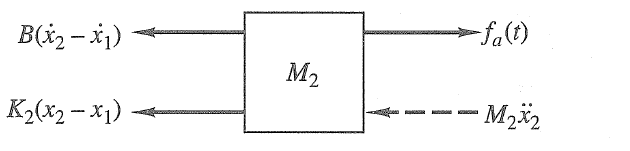
\includegraphics[width=0.5\linewidth]{Figuras/Ch05/fig12.PNG}}
\begin{block}{Diagrama de corpo livre}
\begin{itemize}
    \item Aplicando a lei de D'Alembert, \textbf{respeitando as direções assumidas}, e considerando que as forças agindo para direita são positivas, obtemos:
$$f_a(t) - M_2\ddot{x}_2 - B(\dot{x}_2 - \dot{x}_1) - K_2(x_2-x_1) = 0$$
Rearranjando os termos, temos:
$$-B\dot{x}_1 - K_2x_1 + M_2\ddot{x}_2 + B\dot{x}_2 + K_2x_2 = f_a(t)$$
\end{itemize}
\end{block}
}

\frame{
\frametitle{Exemplo $\#02$ - sistema com duas massas interconectadas}
\begin{block}{EDOs}
\begin{equation*}
\begin{cases}
M_1\ddot{x}_1 + B\dot{x}_1 + (K_1 + K_2)x_1 - B\dot{x}_2 - K_2x_2= 0 \\
-B\dot{x}_1 - K_2x_1 + M_2\ddot{x}_2 + B\dot{x}_2 + K_2x_2 = f_a(t)
\end{cases}
\end{equation*}
\begin{itemize}
    \item Note que, considerando a massa $M_1$, todos os termos envolvendo o deslocamento $x_1$ e suas derivadas \textbf{possuem o mesmo sinal}. Isto é verdadeiro para sistemas onde as únicas fontes de energia permanentes são associadas à entradas externas.
    \item De modo semelhante, considerando a massa $M_2$, todos os termos envolvendo o deslocamento $x_2$ e suas derivadas \textbf{possuem o mesmo sinal}. 
    \item Observe que nada se pode falar sobre os sinais dos outros termos (da outra massa) envolvendo o deslocamento e suas derivadas, visto que tais sinais dependem da referência usada para definição das variáveis.
\end{itemize}
\end{block}
}

\frame{
\frametitle{Exemplo $\#03$ - sistema com deslocamento relativo}
\centerline{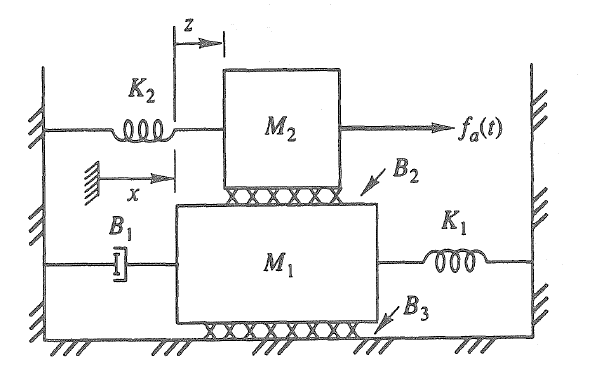
\includegraphics[width=0.4\linewidth]{Figuras/Ch05/fig13.PNG}}
\begin{block}{Problema}
\begin{itemize}
    \item Observe que neste sistema, $\bm{x}$ denota a posição da massa $M_1$ em relação a uma referência \textbf{fixa} e $\bm{z}$ denota o deslocamento da massa $M_2$ em relação a $\bm{M_1}$.
    \item Para a massa $\bm{M_1}$ \textbf{(considere} $\bm{z > x)}$:
    \begin{itemize}
        \item A força devido ao elemento do atrito viscoso $B_2$ é proporcional a velocidade relativa $\dot{z}$ das duas massas. Como $M_2$ está se movendo para direita mais rápido que $M_1$ (por hipótese), então a força em $M_1$ através de $B_2$ tende a puxar a massa para direita.
        \item Os outros elementos ($B_1$, $B_3$, $K_1$ e inércia) se comportam de maneira semelhante ao que já foi visto nos outros exemplos.
    \end{itemize}
\end{itemize}
\end{block}
}

\frame{
\frametitle{Exemplo $\#03$ - sistema com deslocamento relativo}
\centerline{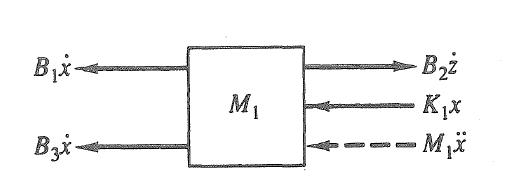
\includegraphics[width=0.5\linewidth]{Figuras/Ch05/fig14.PNG}}
\begin{block}{Diagrama de corpo livre}
\begin{itemize}
    \item Aplicando a lei de D'Alembert, \textbf{respeitando as direções assumidas}, e considerando que as forças agindo para direita são positivas, obtemos:
$$B_2\dot{z} - K_1x - M_1\ddot{x} - B_1\dot{x} - B_3\dot{x} = 0$$
Rearranjando os termos, temos:
$$M_1\ddot{x} + (B_1 + B_3)\dot{x} + K_1x - B_2\dot{z} = 0$$
\end{itemize}
\end{block}
}

\frame{
\frametitle{Exemplo $\#03$ - sistema com deslocamento relativo}
\centerline{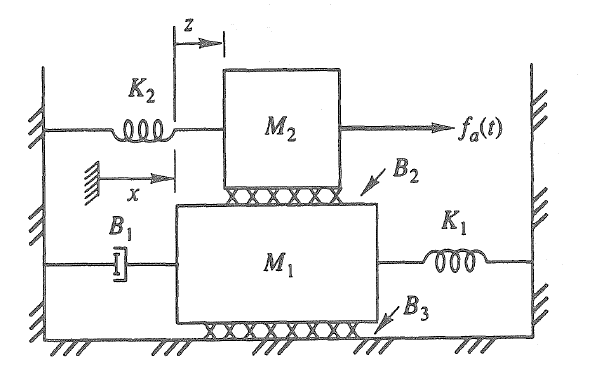
\includegraphics[width=0.35\linewidth]{Figuras/Ch05/fig13.PNG}}
\begin{block}{Problema}
\begin{itemize}
    \item Observe que neste sistema, $\bm{x}$ denota a posição da massa $M_1$ em relação a uma referência \textbf{fixa} e $\bm{z}$ denota o deslocamento da massa $M_2$ em relação a $\bm{M_1}$.
    \item Para a massa $\bm{M_2}$ \textbf{(obrigatoriamente deve-se continuar considerando} $\bm{z > x)}$:
    \begin{itemize}
        \item A deformação da mola $K_2$ é dada por $x+z$.
        \item Além disso, a força de inércia é sempre proporcional a \textbf{aceleração absoluta} $\ddot{x} + \ddot{z}$, e não a aceleração relativa levando em consideração outro corpo em movimento.
        \item Com isso, apenas o elemento $B_2$ é expresso em termo em termos do movimento relativo das duas massas.
    \end{itemize}
\end{itemize}
\end{block}
}

\frame{
\frametitle{Exemplo $\#03$ - sistema com deslocamento relativo}
\centerline{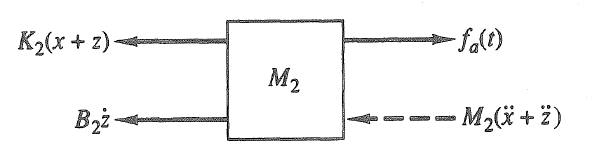
\includegraphics[width=0.6\linewidth]{Figuras/Ch05/fig15.PNG}}
\begin{block}{Diagrama de corpo livre}
\begin{itemize}
    \item Aplicando a lei de D'Alembert, \textbf{respeitando as direções assumidas}, e considerando que as forças agindo para direita são positivas, obtemos:
$$f_a(t) - M_2(\ddot{x} + \ddot{z}) - K_2(x + z) - B_2\dot{z} = 0$$
Rearranjando os termos, temos:
$$M_2\ddot{x} + K_2x + M_2\ddot{z} + B_2\dot{z} + K_2z = f_a(t)$$
\end{itemize}
\end{block}
}

\frame{
\frametitle{Exemplo $\#03$ - sistema com deslocamento relativo}
\begin{block}{EDOs}
\begin{equation*}
\begin{cases}
M_1\ddot{x} + (B_1 + B_3)\dot{x} + K_1x - B_2\dot{z} = 0 \\
M_2\ddot{x} + K_2x + M_2\ddot{z} + B_2\dot{z} + K_2z = f_a(t)
\end{cases}
\end{equation*}
\begin{itemize}
    \item Os mesmos comentários sobre os \textbf{sinais} nas equações de força que foram feitos no exemplo anterior, \textbf{continuam valendo} quando variáveis de deslocamento relativo são usadas.
\end{itemize}
\end{block}
}

\frame{
\frametitle{Exemplo $\#04$ - sistema com polia ideal}
\centerline{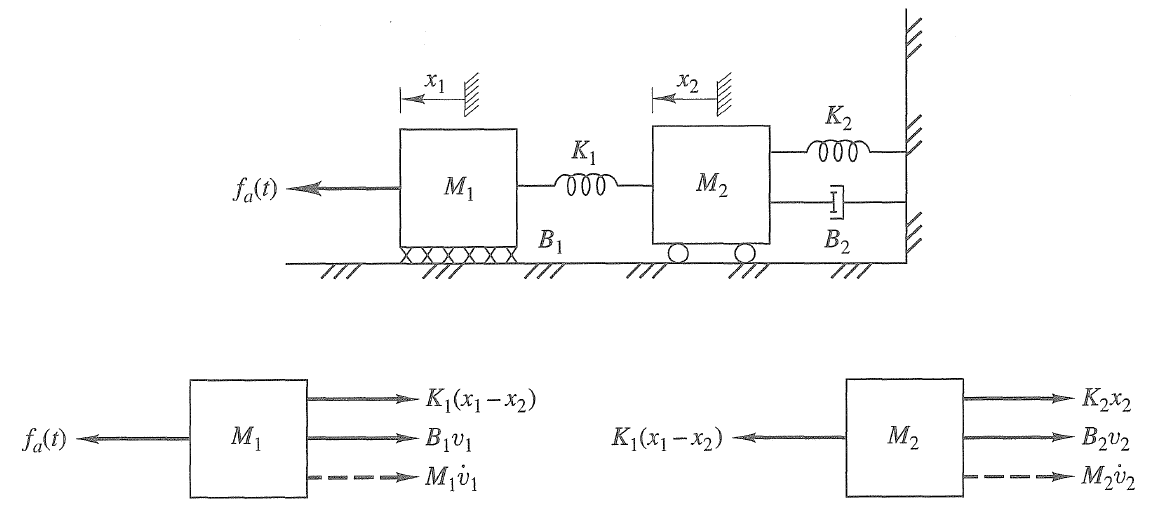
\includegraphics[width=0.8\linewidth]{Figuras/Ch05/fig16.PNG}}
\begin{block}{Diagrama de corpo livre}
\begin{itemize}
    \item Para efeito de observação, considere primeiro o sistema acima sem o uso de uma polia ideal. Utilizando todas as técnicas já estudadas, podemos obter o modelo do sistema como sendo:
\end{itemize}
\begin{equation*}
\begin{cases}
M_1\dot{v_1} + B_1v_1 + K_1(x_1 - x_2) = f_a(t) \\
M_2\dot{v_2} + B_2v_2 + K_2x_2 = K_1(x_1-x_2)
\end{cases}
\end{equation*}
\end{block}
}

\frame{
\frametitle{Exemplo $\#04$ - sistema com polia ideal}
\centerline{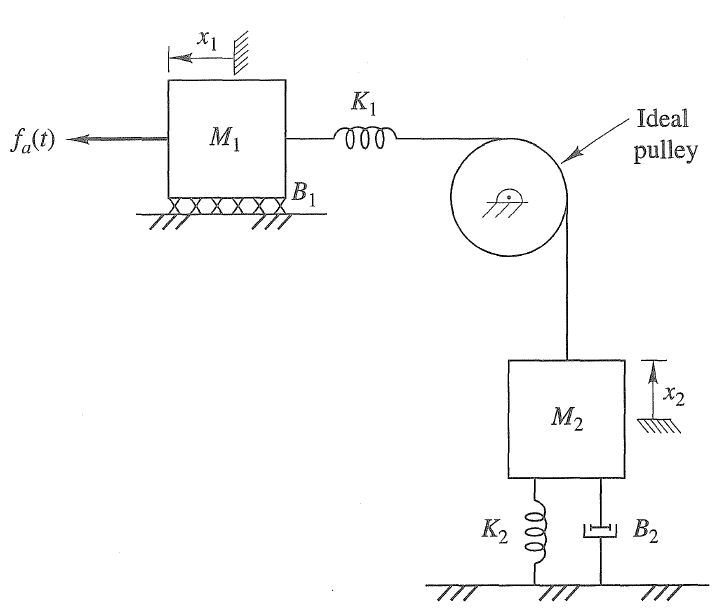
\includegraphics[width=0.4\linewidth]{Figuras/Ch05/fig17.PNG}}
\begin{block}{Problema}
\begin{itemize}
    \item Uma \textbf{polia} pode ser usada para mudar a direção do movimento em um sistema mecânico translacional (parte do sistema se move horizontalmente, e a outra parte \textbf{verticalmente}).
    \item Consideraremos aqui uma polia \textbf{ideal}, que não possui massa nem atrito. Além disso, o cabo da polia não influencia no movimento (cabo e cilindro possuem a mesma velocidade).
    \end{itemize}
\end{block}
}

\frame{
\frametitle{Exemplo $\#04$ - sistema com polia ideal}
\centerline{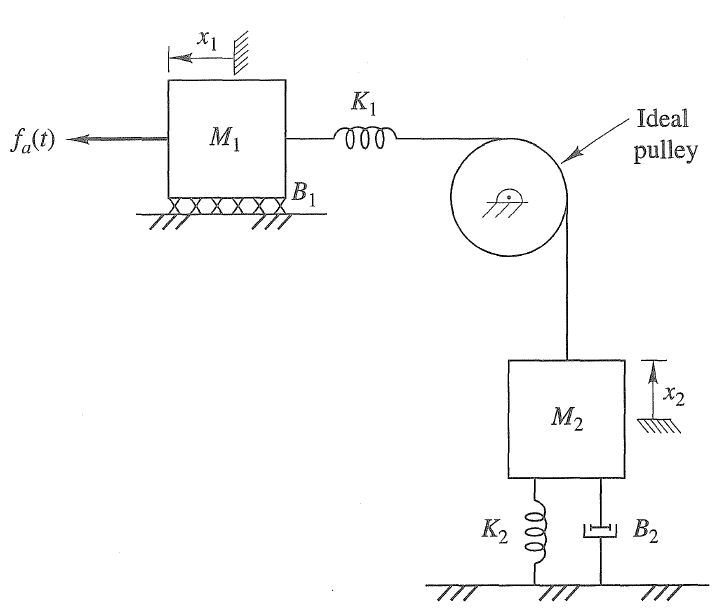
\includegraphics[width=0.4\linewidth]{Figuras/Ch05/fig17.PNG}}
\begin{block}{Problema}
\begin{itemize}
    \item Para a massa $\bm{M_1}$, o diagrama de corpo livre permanece o mesmo.
    \item Para a massa $\bm{M_2}$, assumindo que a polia seja ideal, a força exercida por $K_1$ passa pelo cabo e é exercida diretamente em $M_2$ (o cabo não muda a magnitude desta força, apenas muda a sua direção para cima). Devemos lembrar de incluir a \textbf{força gravitacional}, já que $M_2$ se move verticalmente.
\end{itemize}
\end{block}
}

\frame{
\frametitle{Exemplo $\#04$ - sistema com polia ideal}
\centerline{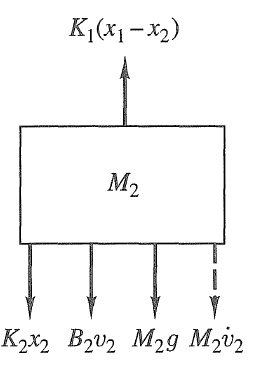
\includegraphics[width=0.25\linewidth]{Figuras/Ch05/fig18.PNG}}
\begin{block}{Diagrama de corpo livre}
\begin{itemize}
    \item Aplicando a lei de D'Alembert, \textbf{respeitando as direções assumidas}, e considerando que as forças agindo para baixa são positivas, obtemos:
\end{itemize}
$$M_2\dot{v_2} + B_2v_2 + K_2x_2 + M_2g = K_1(x_1-x_2)$$
\end{block}
}

\frame{
\frametitle{Exemplo $\#04$ - sistema com polia ideal}
\begin{block}{Comparação das soluções}
\begin{itemize}
    \item Perceba que as duas soluções são idênticas, com exceção da presença da \textbf{força gravitacional} $M_2g$.
    \item Para $(x_1 - x_2) > 0$, temos uma tração na mola e para $(x_1 - x_2) < 0$, temos uma compressão na mola. O primeiro exemplo é \textbf{válido} para quaisquer valores de $x_1$ e $x_2$.
    \item Perceba que isto não pode ser verdade no sistema onde a polia é considerada. Caso tenhamos $(x_1 - x_2) < 0$ o diagrama de corpo livre indicaria uma força para baixo em $M_2$, o que tenderia a separar os dois corpos, o que é \textbf{fisicamente impossível}. 
\end{itemize}
\end{block}
}

\frame{
\frametitle{Exemplo $\#05$ - sistema com elementos em paralelo}
\centerline{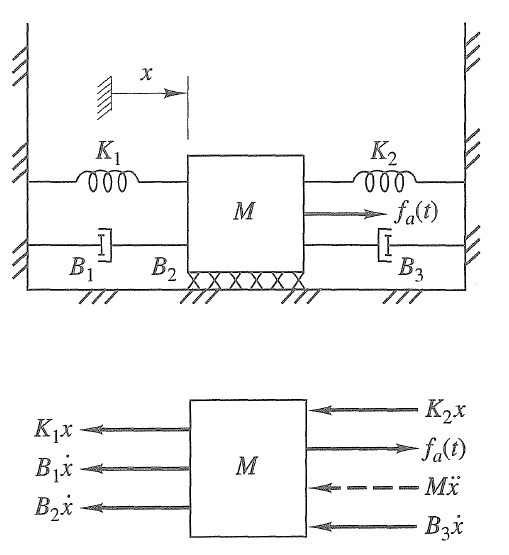
\includegraphics[width=0.35\linewidth]{Figuras/Ch05/fig19.PNG}}
\begin{block}{Diagrama de corpo livre}
$$M \ddot{x} + (B_1 + B_2 + B_3) \dot{x} + (K_1 + K_2)x = f_a(t)$$
Considerando $\boxed{K_{eq} = K_1 + K_2}$ e $\boxed{B_{eq} = B_1 + B_2 + B_3}$, temos:
$$M \ddot{x} + B_{eq} \dot{x} + K_{eq}x = f_a(t)$$
\end{block}
}

\frame{
\frametitle{Exemplo $\#06$ - sistema com elementos em série}
\centerline{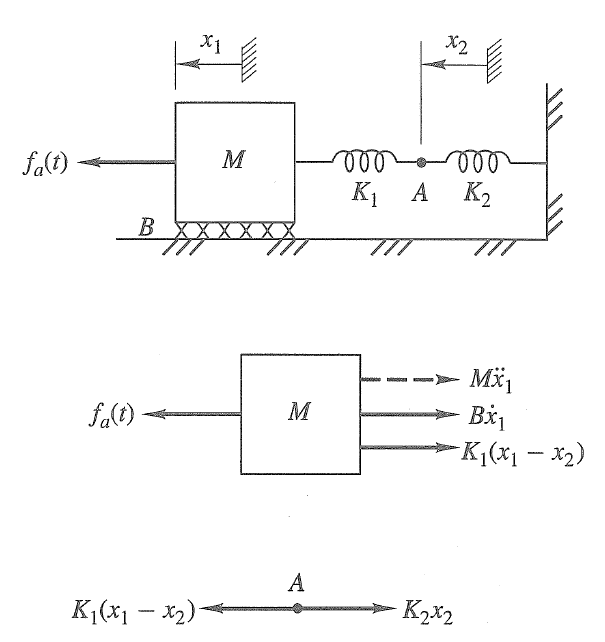
\includegraphics[width=0.45\linewidth]{Figuras/Ch05/fig20.PNG}}
\begin{block}{Diagrama de corpo livre}
\begin{equation*}
\begin{cases}
M \ddot{x}_1 + B \dot{x}_1 + K_1(x_1-x_2) = f_a(t) \\
K_2x_2 = K_1(x_1-x_2)
\end{cases}
\end{equation*}
\end{block}
}

\frame{
\frametitle{Exemplo $\#06$ - sistema com elementos em série}
\begin{block}{Conclusão}
Isolando $x_2$ na segunda equação, obtemos:
$$x_2 = \Big(\dfrac{K_1}{K_1+K_2}\Big)x_1$$
Substituindo $x_2$ na primeira equação, temos:
$$M \ddot{x}_1 + B \dot{x}_1 + K_1\Big[1 - \dfrac{K_1}{K_1+K_2}\Big]x_1 = f_a(t)$$
De onde vem:
$$M \ddot{x}_1 + B \dot{x}_1 + \dfrac{K_1K_2}{K_1+K_2}x_1 = f_a(t)$$
$$\boxed{K_{eq} = \dfrac{K_1K_2}{K_1+K_2}}$$
\end{block}
}

\frame{
\frametitle{Exercícios}
\begin{block}{}
01. Para o sistema mostrado abaixo (à esquerda), desenhe o diagrama de corpo livre e modele-o.

\vspace{0.5cm}

02. Repita para o sistema mostrado à direita.
\end{block}
\centerline{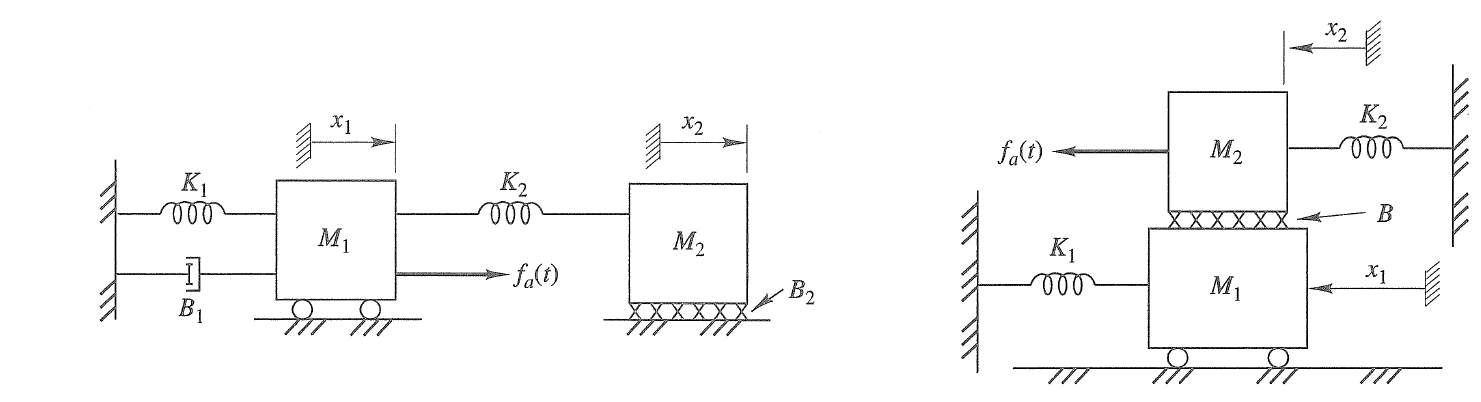
\includegraphics[width=1.1\linewidth]{Figuras/Ch05/fig21.PNG}}
}

\frame{
\frametitle{Referências e exercícios complementares}
\begin{itemize}
\item CLOSE, Charles M.; FREDERICK, Dean K.; NEWELL, Jonathan C. Modeling and Analysis of Dynamic Systems, 3 ed. John Wiley \& Sons, 2003.
\end{itemize}
\centering{\alert{Página 39 - \textbf{Capítulo 2}}} \\
}








